\documentclass[a4paper]{article}

\usepackage{preamble}
\usepackage{tipa}
\addbibresource{references/refs.bib}

\usetikzlibrary{automata,positioning}

\newcommand{\blank}{\text{\textvisiblespace}}
\newcommand{\el}[1]{\text{\textopencorner}#1\text{\textcorner}}
\newcommand{\RPrf}[1]{\textsf{RPrf}(#1)}
\newcommand{\Prf}[1]{\textsf{Prf}(#1)}

\title{LOG111 - A5}
\author{Frank Tsai}

\begin{document}

\maketitle

\section{}
Assume that the natural number $n$ is encoded as a string of $n$ I's; the two arguments are delimited by a single $\blank$.
The machine works as follows.

The machine skips over $x$ ($q_0$); then it sweeps through the content of $y$ while keeping track of the parity of the number of $I$'s in $y$ ($q_1$ and $q_4$).

After sweeping through the content of $y$, if the machine ends up in state $q_1$ ($y$ is even) then it erases $y$ and replaces the delimiter with $I$, effectively adding 1 to $x$; if the machine ends up in state $q_4$ ($y$ is odd) then it erases the input, producing $0$.

\begin{center}
  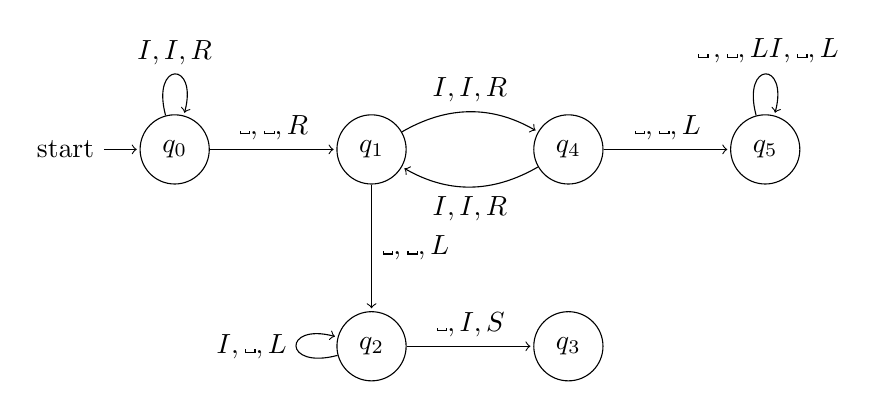
\begin{tikzpicture}[shorten >=1pt,node distance=2.5cm,on grid,auto]
    \node[state,initial] (0) {$q_0$};
    \node[state,right=of 0] (1) {$q_1$};
    \node[state,below=of 1] (2) {$q_2$};
    \node[state,right=of 2] (3) {$q_3$};
    \node[state,right=of 1] (4) {$q_4$};
    \node[state,right=of 4] (5) {$q_5$};
    \path[->]
    (0) edge [loop above] node {$I,I,R$} (0)
    (0) edge node {$\blank,\blank,R$} (1)
    (1) edge node {$\blank,\blank,L$} (2)
    (2) edge [loop left] node {$I,\blank,L$} (2)
    (2) edge node {$\blank,I,S$} (3)
    (1) edge [bend left] node {$I,I,R$} (4)
    (4) edge [bend left] node {$I,I,R$} (1)
    (4) edge node {$\blank,\blank,L$} (5)
    (5) edge [loop above] node {$\begin{matrix}\blank,\blank,L\\I,\blank,L\end{matrix}$} (5);
  \end{tikzpicture}
\end{center}

We can define $f$ by $f(x,y) := \texttt{test}(\texttt{even}(y),x+1,0)$; this is a primitive recursive function since each of its constituents is primitive recursive.

\section{}
Suppose that $\psi(x)$ is a truth definition in PA.
As $\lnot\psi(x)$ is a monadic formula in PA, there is a sentence $\gamma$ such that $\text{PA} \vdash \gamma \leftrightarrow \lnot\psi(\el{\gamma})$ by the fixed-point lemma, but $\text{PA} \vdash \gamma \leftrightarrow \psi(\el{\gamma})$ by definition.
Thus, assuming that PA is consistent truth definition does not exist.

\section{}
Suppose that $X$ is a recursive set separating $A$ and $B$.
By hypothesis, its characteristic function $\chi_X$ is representable by a formula $\chi(x,y)$; by the fixed-point lemma there is a sentence $\gamma$ such that $T \vdash \gamma \leftrightarrow \lnot\chi(\el{\gamma},1)$.

If $\el{\gamma} \in X$ then $T \vdash \chi(\el{\gamma},1)$ by representability; thus, $T \vdash \lnot\gamma$, implying that $\el{\gamma} \in B$.
This contradicts $X \cap B = \varnothing$.
Conversely, if $\el{\gamma} \notin X$ then $T \vdash \forall y(0 \neq y \to \lnot\chi(\el{\gamma},y))$ by representability.
Clearly $T \vdash 0 \neq 1$, so $T \vdash \lnot\chi(\el{\gamma},1)$; thus, $T \vdash \gamma$, but this means $\el{\gamma} \in A$, contradicting $A \cap (\mathbb{N} \setminus X) = \varnothing$.

%\printbibliography

\end{document}
